%!TEX root = ../thesis.tex

\begin{figure}
\centering
\begin{subfigure}{.5\textwidth}
  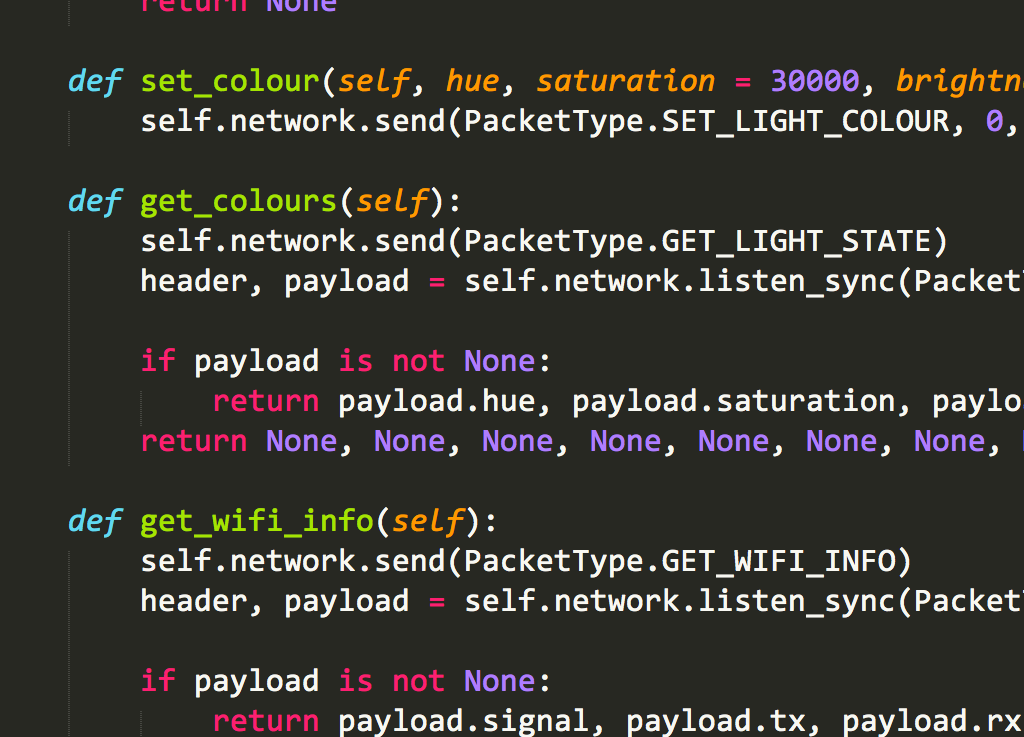
\includegraphics[width=.95\linewidth]{../images/code-visualisations/syntax-highlighting.png}
  \caption{Syntax Highlighting}
  \label{fig:syntax-highlighting}
\end{subfigure}%
\begin{subfigure}{.5\textwidth}
  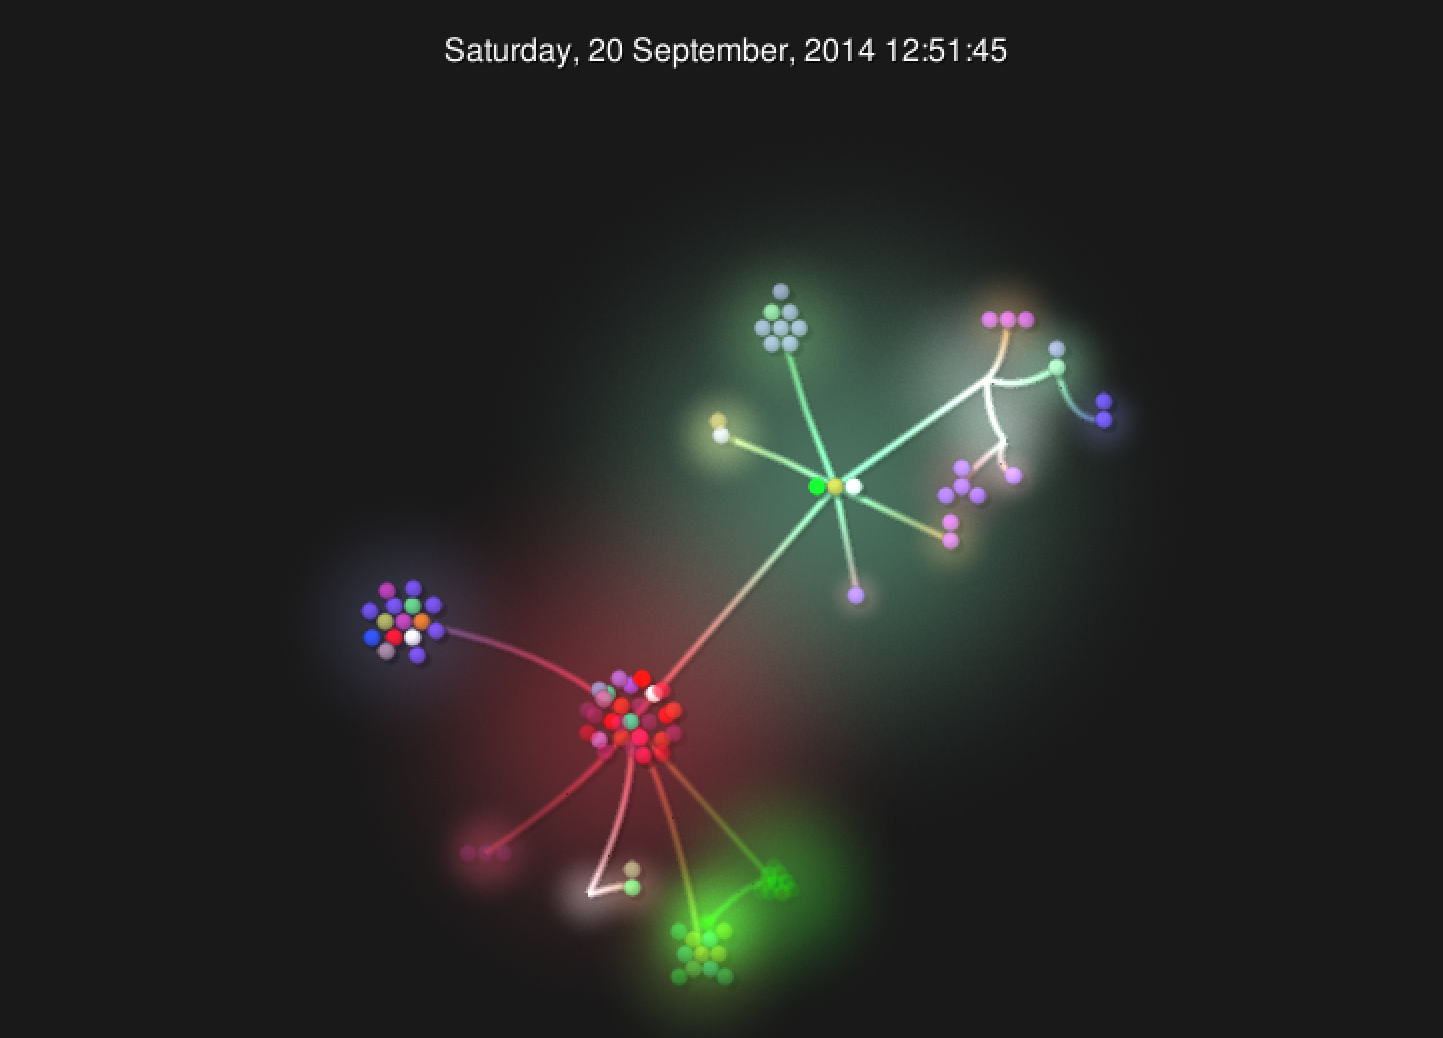
\includegraphics[width=.95\linewidth]{../images/code-visualisations/gource.png}
  \caption{Gource \protect\cite{Caudwell2010}}
  \label{fig:gource}
\end{subfigure}\\
\vspace{5mm}
\begin{subfigure}{.5\textwidth}
  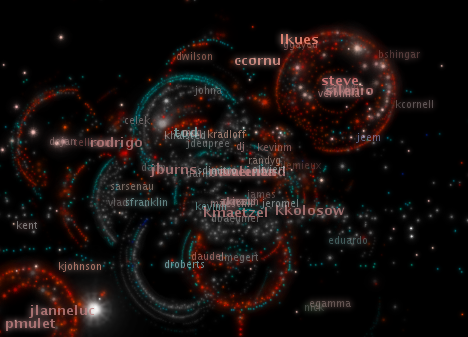
\includegraphics[width=.95\linewidth]{../images/code-visualisations/code-swarm.png}
  \caption{Code Swarm \protect\cite{Ogawa2012}}
  \label{fig:code-swarm}
\end{subfigure}%
\begin{subfigure}{.5\textwidth}
  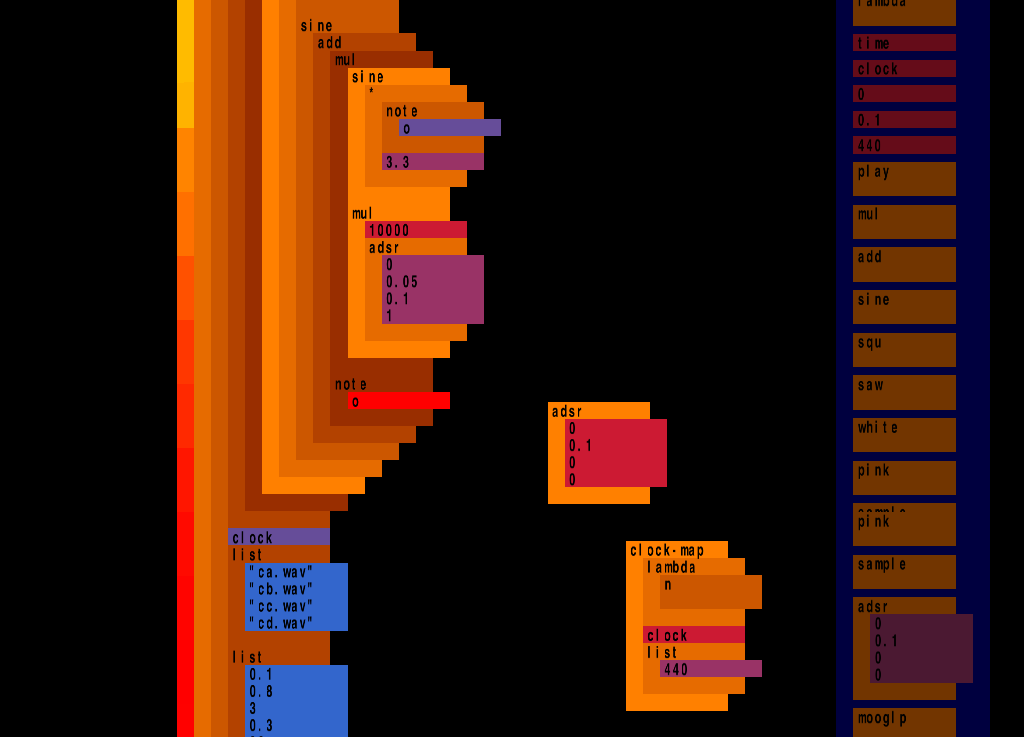
\includegraphics[width=.95\linewidth]{../images/code-visualisations/scheme-bricks.png}
  \caption{Scheme Bricks \protect\cite{McLean2010a}}
  \label{fig:scheme-bricks}
\end{subfigure}

\caption[Existing software visualisations techniques]{Existing software visualisations techniques.}
\label{fig:code-visualisations}
\end{figure}